% This file was created with tikzplotlib v0.10.1.
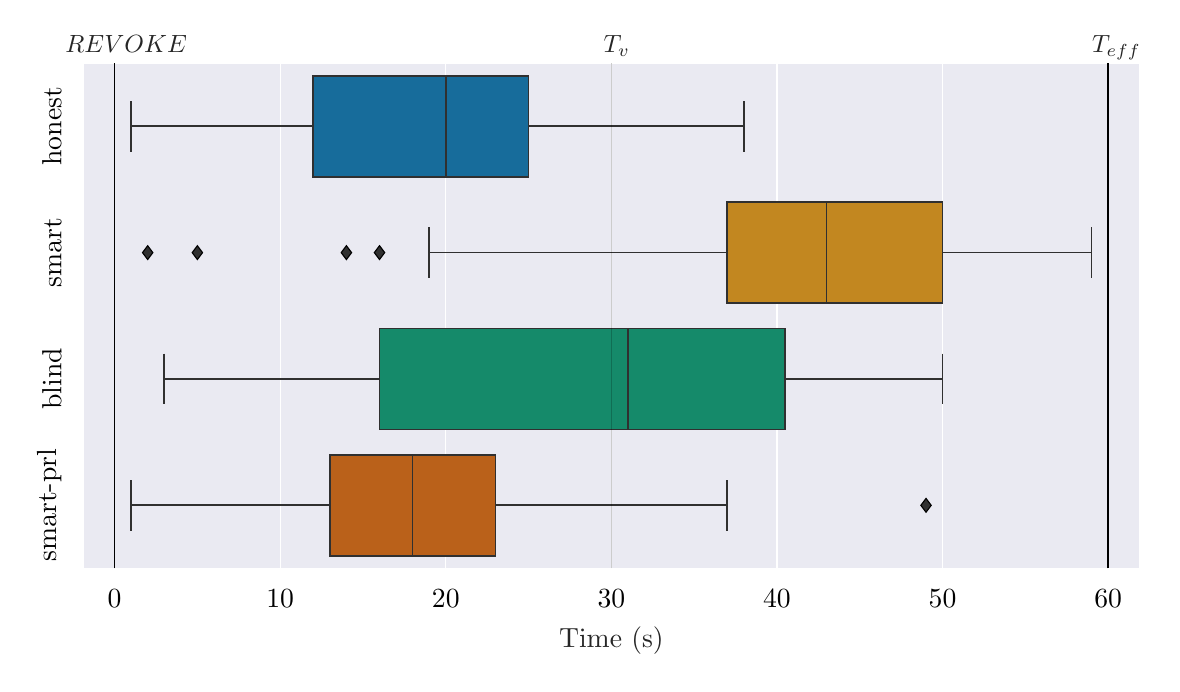
\begin{tikzpicture}

\definecolor{chocolate1869726}{RGB}{186,97,26}
\definecolor{darkgoldenrod19413532}{RGB}{194,135,32}
\definecolor{darkslategray38}{RGB}{38,38,38}
\definecolor{darkslategray48}{RGB}{48,48,48}
\definecolor{lavender234234242}{RGB}{234,234,242}
\definecolor{seagreen21138106}{RGB}{21,138,106}
\definecolor{teal23108155}{RGB}{23,108,155}

\begin{axis}[
clip=false,
axis background/.style={fill=lavender234234242},
axis line style={white},
height=8cm,
minor xtick={},
minor ytick={},
tick align=outside,
width=15cm,
x grid style={white},
xlabel=\textcolor{darkslategray38}{Time (s)},
xmajorgrids,
xmajorticks=true,
xmin=-1.9, xmax=61.9,
xtick style={color=darkslategray38,draw=none},
xtick={-10,0,10,20,30,40,50,60,70},
y dir=reverse,
y grid style={white},
ymajorticks=true,
ymin=-0.5, ymax=3.5,
ytick style={color=darkslategray38,draw=none},
ytick={0,1,2,3},
yticklabel style={rotate=90.0},
yticklabels={honest,smart,blind,smart-prl}
]
\path [draw=darkslategray48, fill=teal23108155, semithick]
(axis cs:12,-0.4)
--(axis cs:12,0.4)
--(axis cs:25,0.4)
--(axis cs:25,-0.4)
--(axis cs:12,-0.4)
--cycle;
\path [draw=darkslategray48, fill=darkgoldenrod19413532, semithick]
(axis cs:37,0.6)
--(axis cs:37,1.4)
--(axis cs:50,1.4)
--(axis cs:50,0.6)
--(axis cs:37,0.6)
--cycle;
\path [draw=darkslategray48, fill=seagreen21138106, semithick]
(axis cs:16,1.6)
--(axis cs:16,2.4)
--(axis cs:40.5,2.4)
--(axis cs:40.5,1.6)
--(axis cs:16,1.6)
--cycle;
\path [draw=darkslategray48, fill=chocolate1869726, semithick]
(axis cs:13,2.6)
--(axis cs:13,3.4)
--(axis cs:23,3.4)
--(axis cs:23,2.6)
--(axis cs:13,2.6)
--cycle;
\addplot [semithick, darkslategray48]
table {%
12 0
1 0
};
\addplot [semithick, darkslategray48]
table {%
25 0
38 0
};
\addplot [semithick, darkslategray48]
table {%
1 -0.2
1 0.2
};
\addplot [semithick, darkslategray48]
table {%
38 -0.2
38 0.2
};
\addplot [semithick, darkslategray48]
table {%
37 1
19 1
};
\addplot [semithick, darkslategray48]
table {%
50 1
59 1
};
\addplot [semithick, darkslategray48]
table {%
19 0.8
19 1.2
};
\addplot [semithick, darkslategray48]
table {%
59 0.8
59 1.2
};
\addplot [black, mark=diamond*, mark size=2.5, mark options={solid,fill=darkslategray48}, only marks]
table {%
2 1
5 1
16 1
14 1
};
\addplot [semithick, darkslategray48]
table {%
16 2
3 2
};
\addplot [semithick, darkslategray48]
table {%
40.5 2
50 2
};
\addplot [semithick, darkslategray48]
table {%
3 1.8
3 2.2
};
\addplot [semithick, darkslategray48]
table {%
50 1.8
50 2.2
};
\addplot [semithick, darkslategray48]
table {%
13 3
1 3
};
\addplot [semithick, darkslategray48]
table {%
23 3
37 3
};
\addplot [semithick, darkslategray48]
table {%
1 2.8
1 3.2
};
\addplot [semithick, darkslategray48]
table {%
37 2.8
37 3.2
};
\addplot [black, mark=diamond*, mark size=2.5, mark options={solid,fill=darkslategray48}, only marks]
table {%
49 3
};
\addplot [semithick, black]
table {%
0 3.5
0 -0.5
};
\addplot [semithick, black, opacity=0.2]
table {%
30 3.5
30 -0.5
};
\addplot [semithick, black]
table {%
60 3.5
60 -0.5
};
\addplot [semithick, darkslategray48]
table {%
20 -0.4
20 0.4
};
\addplot [semithick, darkslategray48]
table {%
43 0.6
43 1.4
};
\addplot [semithick, darkslategray48]
table {%
31 1.6
31 2.4
};
\addplot [semithick, darkslategray48]
table {%
18 2.6
18 3.4
};
\draw (axis cs:-3.5,-0.58) node[
  scale=0.9,
  anchor=base west,
  text=darkslategray38,
  rotate=0.0
]{$REVOKE$};
\draw (axis cs:29,-0.58) node[
  scale=0.9,
  anchor=base west,
  text=darkslategray38,
  rotate=0.0
]{$T_{v}$};
\draw (axis cs:58.5,-0.58) node[
  scale=0.9,
  anchor=base west,
  text=darkslategray38,
  rotate=0.0
]{$T_{eff}$};
\end{axis}

\end{tikzpicture}
